% -*- mode: latex; mode: linkd; mode: auto-fill; mode: flyspell;-*-
\chapter{Design and Implementation}
\label{chap-five}


% Introduction

% Discuss what this chapter will focus on and dive in.
The purpose of this chapter is three fold: it discusses the motivations
that governed the design of the system, such as using the
BioBike\cite{journals/bioinformatics/MassarTES05} chassis and using
frames as a data structure to represent ACT-R based cognitive models;
it describes the work flow of the system that enables users to build
and share models and finally it discusses in detail a medium scale
model that was built as a proof of concept.

\section{Problem Definition for Coglaborate}

% This is where I have to discuss what coglaborate is trying to
% achieve 

The primary goal of the Coglaborate system is to provide a
collaborative tool-based environment for the computational cognitive
modeling community. Currently there are no known environments that
provide this facility. Apart from providing collaboration, Coglaborate
also intends to achieve a number of secondary goals:

% Sand boxing 
% Resource sharing
% Tool integration
% Knowledge agglomeration
\begin{itemize}
\item \emph{A sand boxed environment}: Currently there are number of
  interesting extensions to ACT-R. But occasionally it might be
  difficult for the users of the extensions to set them up. But with a
  sand boxed environment, users can connect to it and use the module
  with out any setup. This has a number of advantages, firstly the
  users do not have to keep track of the version of the extension and
  they can focus on completing their tasks rather than having to
  tinker around the computer.
\item \emph{Resource Sharing}: When we refer to resource sharing we refer to
  sharing hardware. With a web based platform that runs on a powerful
  computer researchers can simulate models that require excessive
  computational power and time.
\item \emph{Tool Integration}: If there are computational tools that a model
  would like to utilize they can be hooked in. For example the R
  statistical environment can be accessed by hooking in a
  library. Once loaded in a number of users would be able to access
  the facilities provided by it.
\item \emph{Knowledge Agglomeration}: As users model various aspects
  of cognition we would be able to build a repository that reflects
  the state of the field.
\end{itemize}

\section{Design Decisions}
% Design Decisions
%       - Why biobike
There were two major decisions that influenced the design of the
project: firstly the use of the BioBike chassis as a platform to
mount the ACT-R framework; and secondly the use of frames as means to
represent ACT-R based cognitive models in the shared memory. This
section discusses the alternatives that were analyzed and the reasons
why we chose to stick with the existing decisions.

\subsection{Choice of platform}

% Bio bike and the vision that it is originally based on
We chose the BioBike framework as the platform for the system. This
section examines the basis of that decision by analyzing the
capabilities of BioBike. BioBike is an instantiation of
KnowOS\cite{oai:CiteSeerXPSU:10.1.1.75.7132} a concept based on the
view that knowledge could be treated on par as the rest of the
elements that make up a computer system. It is well known fact that
Operating systems provide abstractions to work with the elements of a
system for example, consider a file. An operating system provide
operations using which this file can be renamed, copied, deleted
etc. It also provides further abstractions that allow us to significant
modifications to raw data. The KnowOS vision extends this analogy to
the realm of knowledge. An implementation of the KnowOS consists of
the following layers\cite{oai:CiteSeerXPSU:10.1.1.75.7132}:


\begin{itemize}
\item An knowledge base centered around the frame system
\item An efficient and highly extensible language that provides an
  abstraction to the users to work with the system.
\item A web-based interface to the programming language and to other
  KnowOS services.
\end{itemize}

% Description of biobike
%       - Components
BioBike originally known as BioLingua seeks to provide biologists with
the ability to perform computational biology operations on large data
sets using a simple language. BioBike ties up a number of knowledge
bases transparently using a frame based representation to represent
organisms. Being an implementation of the KnowOS vision it provides
features customized for molecular biologists. These
include\cite{journals/bioinformatics/MassarTES05}

\begin{itemize}
\item A common framework to access genomic, metabolic and experimental data.
\item A general purpose programming language(lisp) customized to
  provide transparent access to the underlying knowledge bases.
\item A highly interactive environment where code can be evaluated and
  its results displayed immediately.
\item A number of general purpose tools that help in analyzing interactions.
\item A wiki through which scientists can collaborate and announce results.
\end{itemize}

% Talk about the style of interaction and the result
The BioBike language is built on top of Common Lisp. Users interact
with the system using a lisp listener. This results in a Unix style
interaction between the system and the user, where the user types in a
command and can see the results of that action immediately. All
listeners of the system share the same workspace as a result they can
share code.

This system provides biologists with: an environment in which they
interact with computer in the same terms as they would interact with
their peers; a uniform framework using which they can access knowledge
from a number of different knowledge bases; a common work area where
data and results can be shared and an environment where external tools
can be integrated.

\subsubsection{Design Choices}

When making the decision about the platform of the system the only
other option we had was to implement a similar system from
scratch. But when considering the capabilities provided by biobike
such as: a live lisp listener; a system for integrating third party
tools; its natural ability to lend support for collaboration and the
robustness of the existing code; made the decision of choosing a
platform a trivial one.

Further benefits of this decision are related to software engineering
aspects. The code for the system is open sourced under the MIT
license and is actively maintained. As a result we would be able to
download updates to the code and apply those changes in a way we see
fit to the system.

\subsection{Choice of structure for representation}
% Introduction
A structured representation of an ACT-R model provides us with an
abstraction. This abstraction gives us a number of capabilities such
as: the ability to share models conveniently; writing an ecosystem of
tools for ACT-R models; the ability to maintain revisions of
models and the ability to extend it in ways not foreseen when the
system was originally designed.

We had to decide between three main choices of structures for
representing an ACT-R model. These are a direct representation of the
model, a semantic network and frames. 

%       - Direct representation: that is store the entire code as some variable
ACT-R models are lisp data structures. Therefore direct representation
of the model would have stored the code for the model as is. The
benefit of the approach lies in the simplicity of the implementation,
which would have involved storing the code as symbols. But this
representation has a number of disadvantages: writing tools for this
representation would be exceptionally hard because the tools would
have to parse the model before being able to perform any operations;
the representation does not allow us to store meta data; it does not
allow us to add capabilities for reuse of the model and finally it
would be quite cumbersome to implement a system of revision control
for this data structure.

%       - Semantic Nets
%         - Describe Semantic nets
An alternative to the direct representation is using semantic networks
to represent ACT-R models. Semantic networks is a notation for
representing knowledge using nodes that usually represent objects,
concepts or situations in a domain and the arcs represent relations
between them\cite{Sowa87, Barr81}. A way to represent ACT-R models
would have represented the model, the productions, conditions and
actions as nodes. Relationships between the nodes would be shown using
arcs that describe the relation between various nodes. The advantages
of using this representation are: tools written for ACT-R can act
directly on the nodes that represent productions and models; this
representation would make it easy to implement facilities for reuse of
productions and we can write queries to determine the type of objects
and inter-relationships. The deficiencies of this representation are
that implementing a system of revision control would be difficult
because we would not be able to represent version information; it
would like the direct representation model we would not be able to add
capabilities of model reuse.


%       - Why frames
% -     Describe frames
% Brief description of other possible structures if I had not used
% frames.

The frame data structure was introduced by Marvin
Minsky\cite{Minsky1974a} in 1975 in one the seminal papers in the area
of knowledge representation. Frames are structures that can represent
objects, situations and concepts. Frames are arranged in a
hierarchical taxonomy where every frame is linked with its parent
frame. The parent frame represents a more general concept than its
child\cite{karp-93}. A frame is made up of a number of slots. Slots
define the properties of the object being represented by the
frame. Slots are sometimes also used to represent relationships
between two frames. This representation provides us with a number of
advantages: Unlike semantic networks we have all related data stored
in a single frame; frames are dynamic and they allow slots and their
values to be updated very easily; since frames are structured writing
tools to help perform various forms of analysis would be easy and
finally in the future frames might help in analyzing more complex
forms of reuse of cognitive models.

% Describe frames in reasonable amount of detail.

% describe why are frames the sweetest things since sliced bread...

\section{System Design}

\begin{figure}[htp]
  \centering
  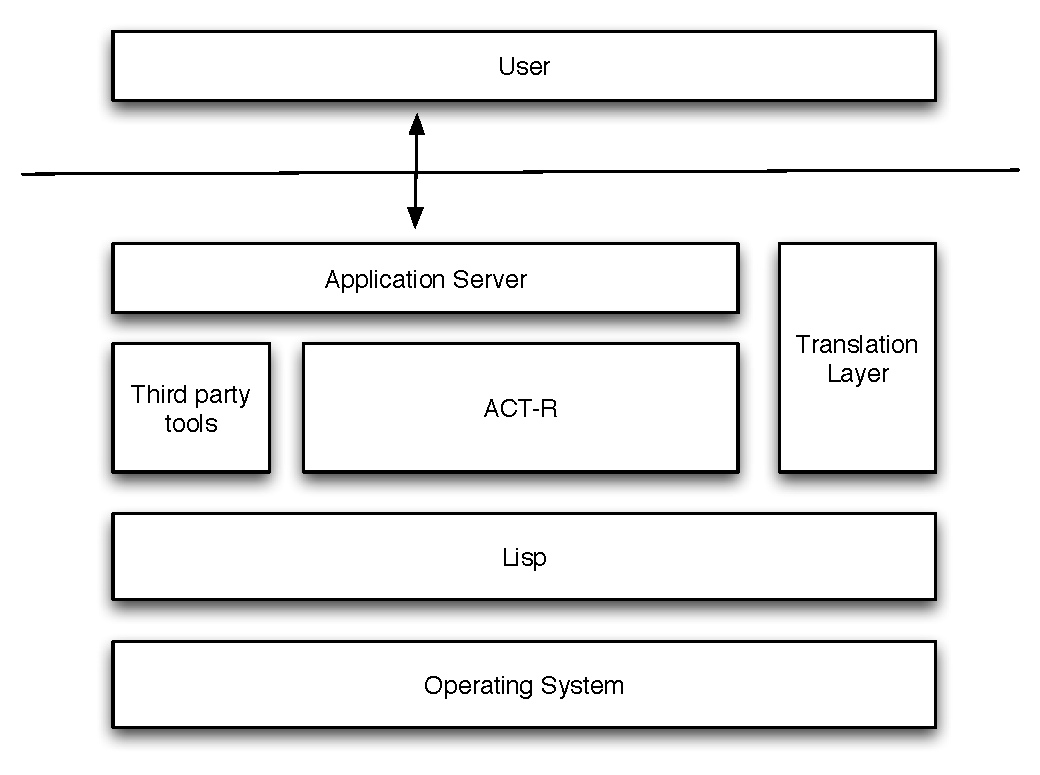
\includegraphics[width=90mm]{SystemOverview}
  \caption{System Design}
  \label{SysOverview}
\end{figure}

This section aims to explain how various components of the system work
together to have the desired effect. Figure \ref{SysOverview} provides
us with a high level of the system.  This section will examine each
component in detail. The system currently runs on a server running
GNU/Linux as a result we have a secure, robust and stable platform to
base our system.

%\subsubsection{Operating System}
% there obviously is no need to introduce the operating system. 
% The system currently runs on a GNU/Linux based machine. 

\subsubsection{Application Server}

% Describe the application server...The places where the request comes
% in and how the code flows.

\subsubsection{Lisp}

% Do I advocate the use of lisp here or do I just describe the version
% being used and its benefits

\subsubsection{Translation Layer}

%Describe what happens here....draw diagrams to show frames from
%various levels...for example frames that represent productions,
%models, actions and conditions. 


\section{Work Flow}

This section illustrates a scenario where a user creates a model and
evaluates it. Another user comes in searches for the model created by
the first user, navigates around its productions and obtains the code for
it. 

\begin{figure}[htp]
  \centering
  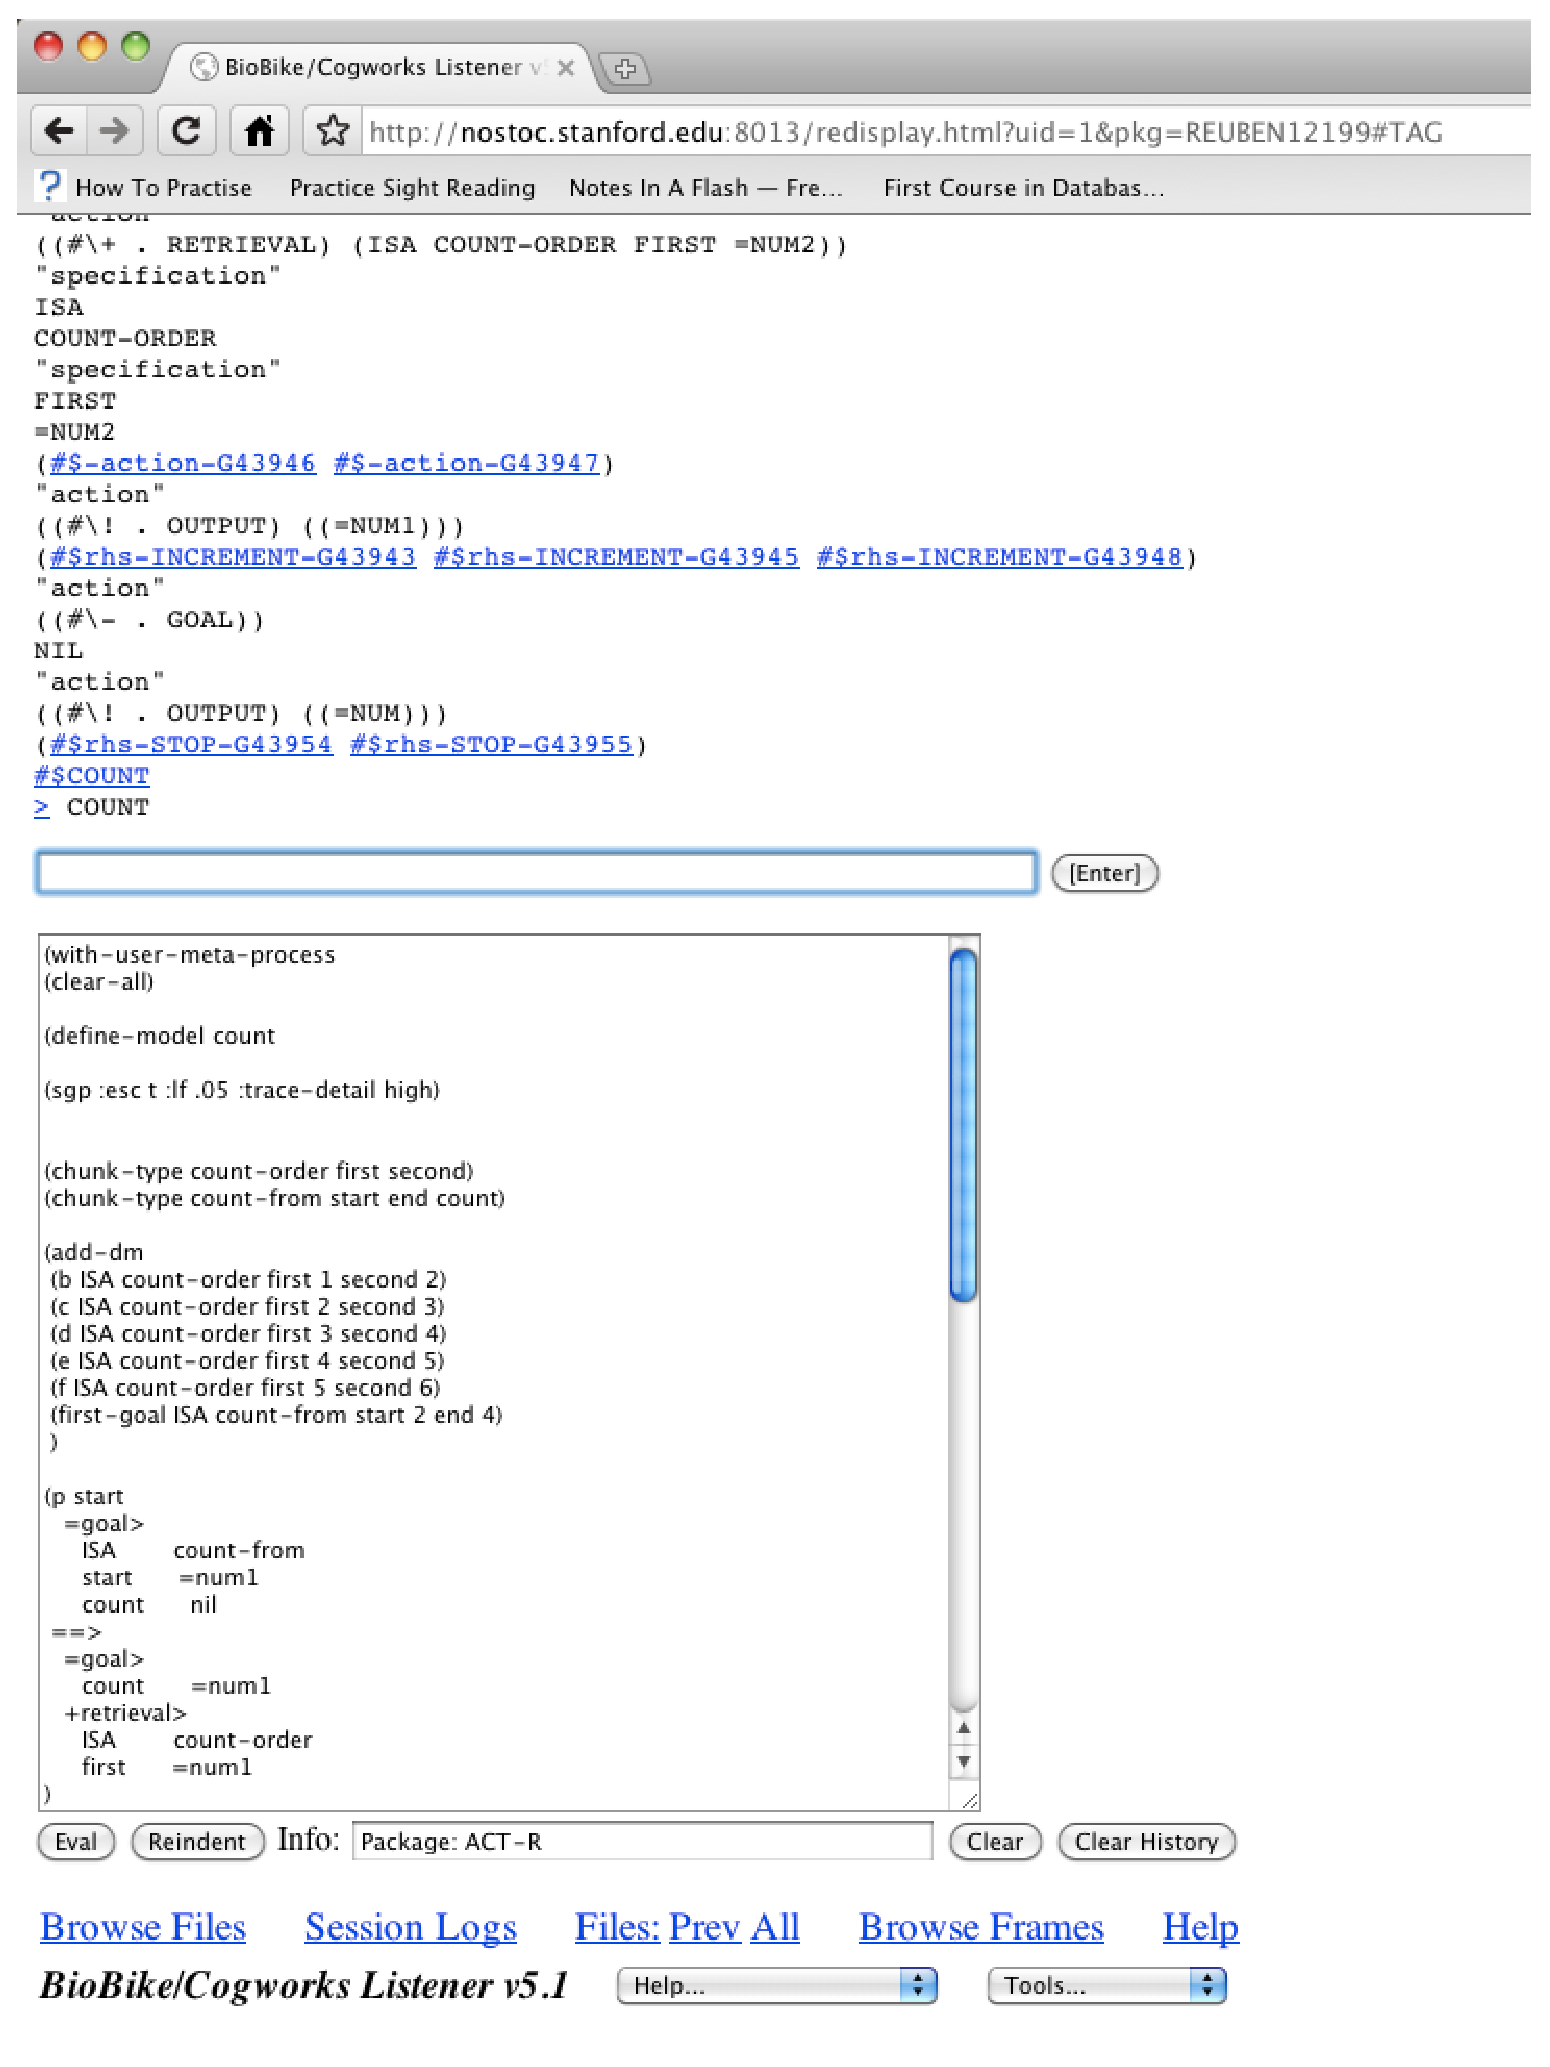
\includegraphics[width=100mm]{UserCreatesModel}
  \caption{A user creates and evaluates a model}
  \label{UserCreatesModel}
\end{figure}

\begin{figure}[htp]
  \centering
  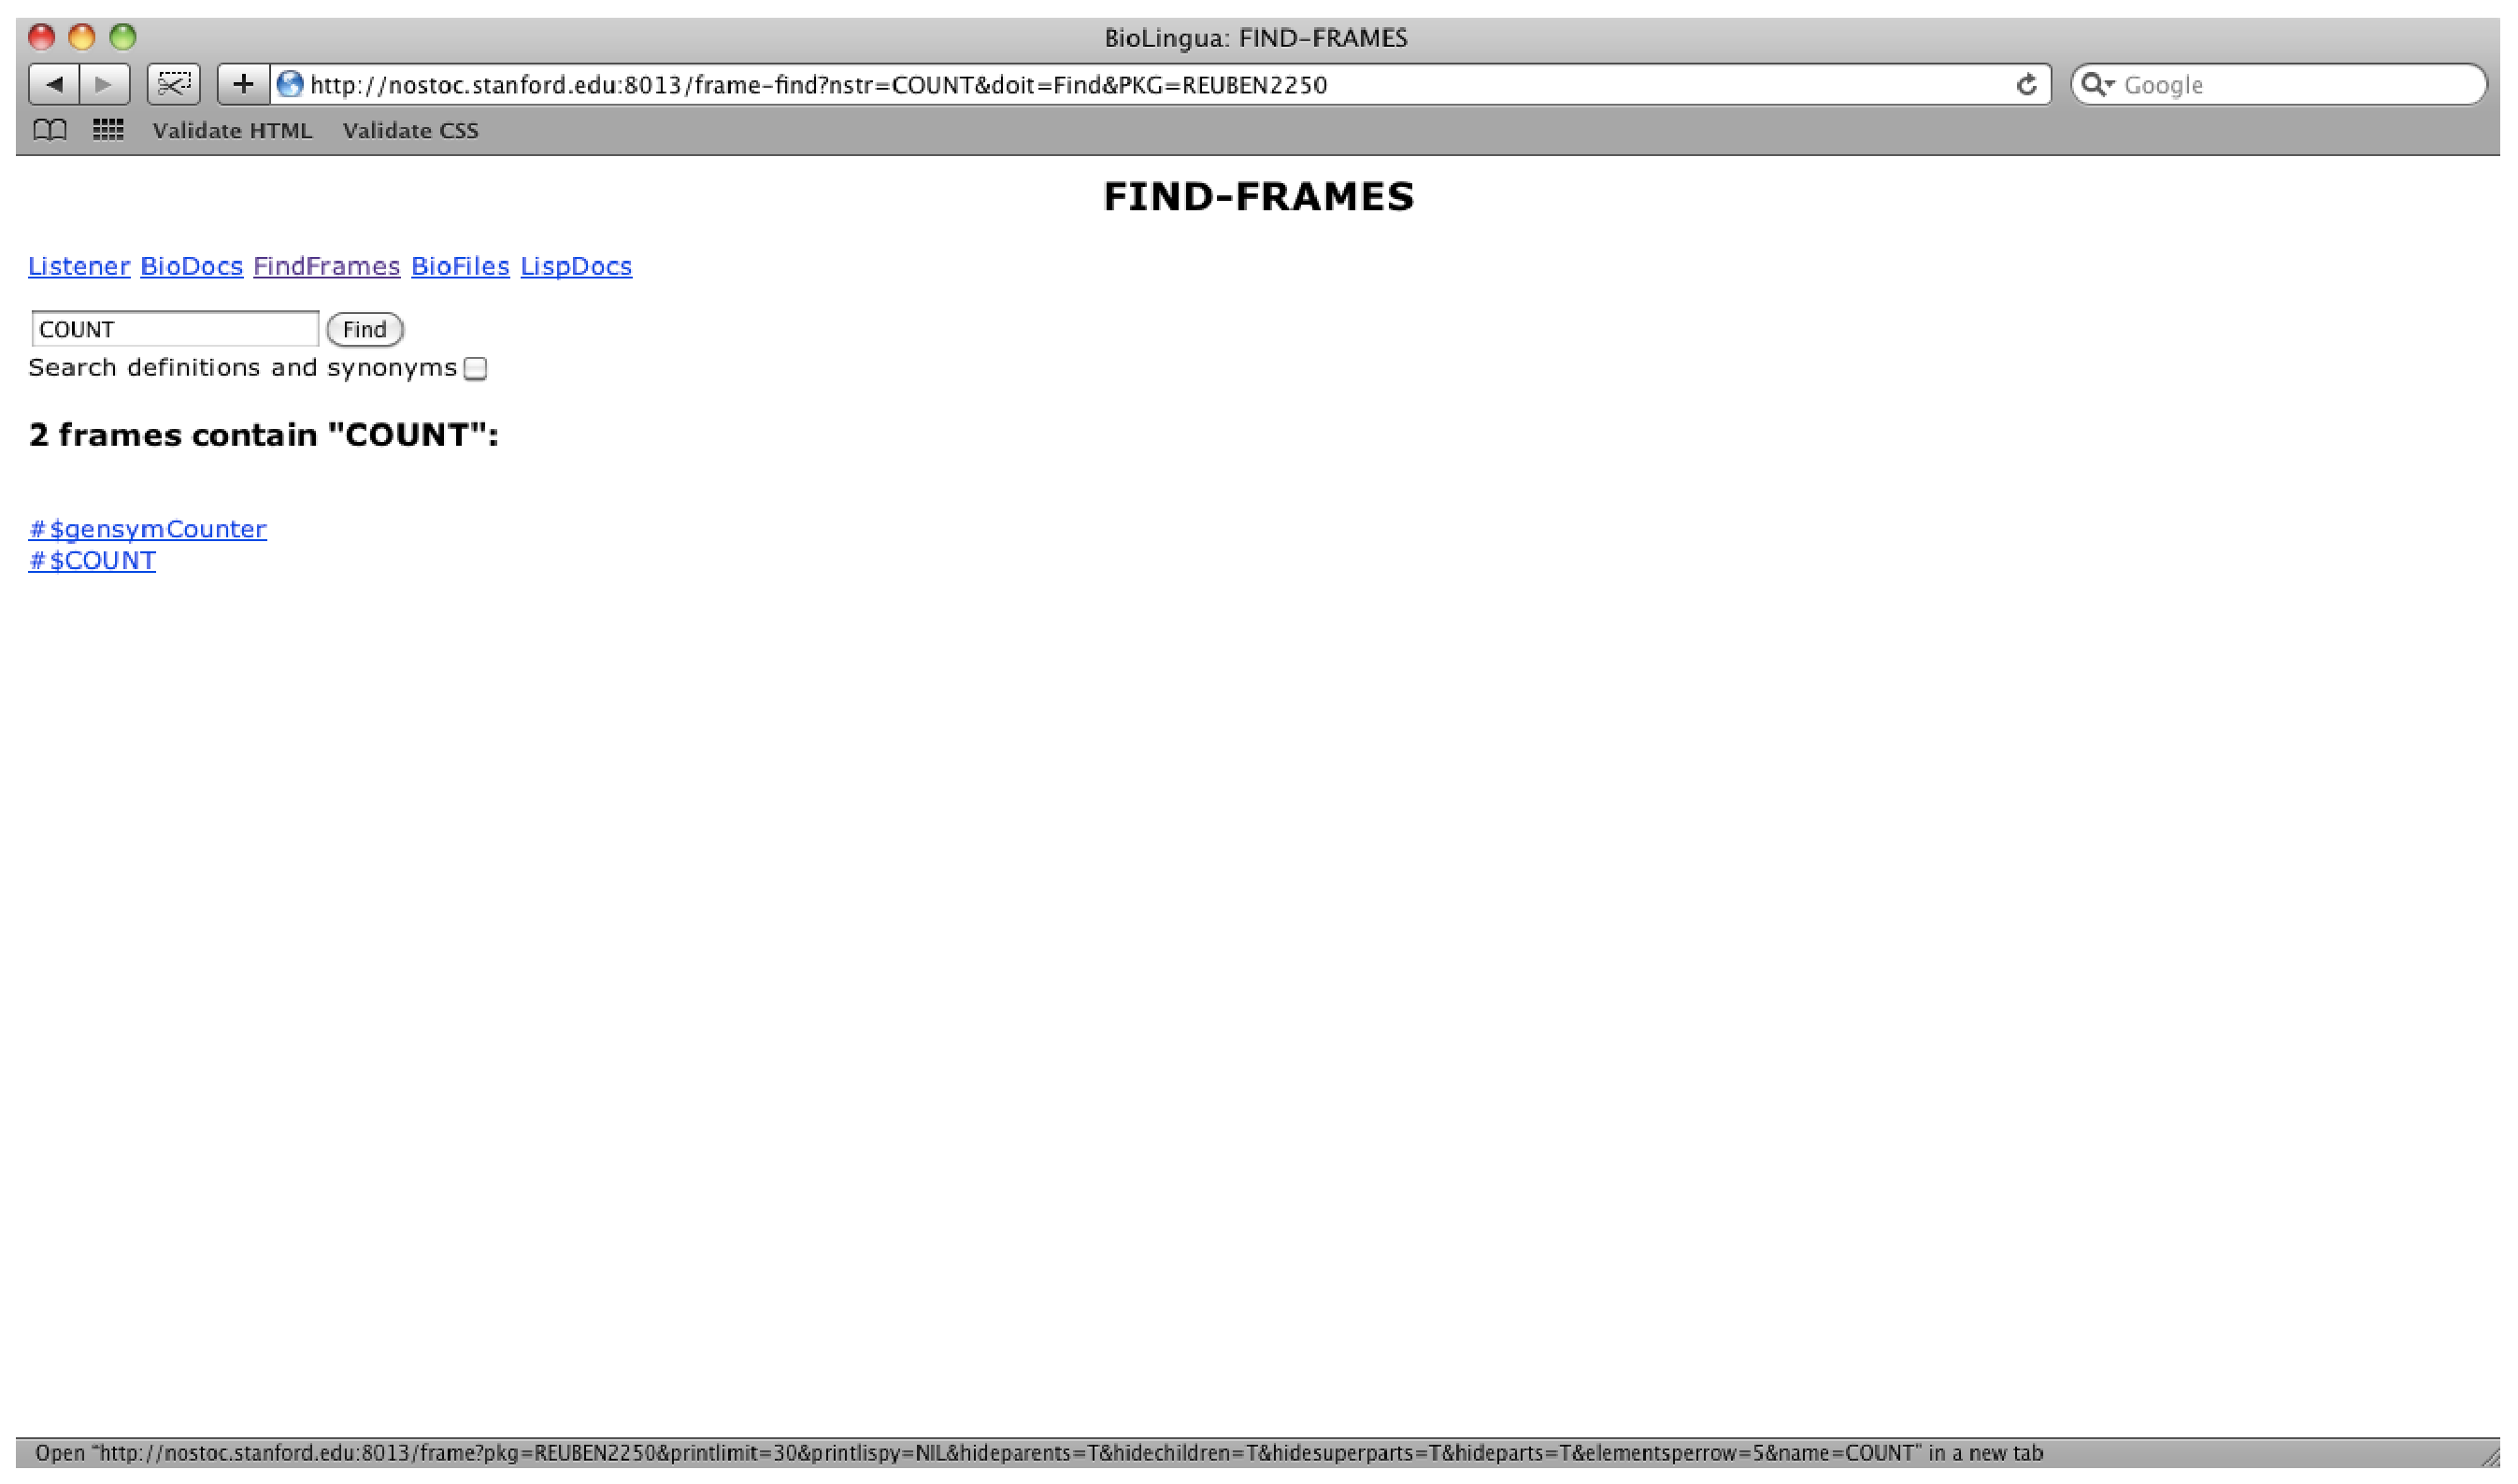
\includegraphics[width=100mm]{SearchForModel}
  \caption{Search results after searching for a model}
  \label{SearchForModel}
\end{figure}

\begin{figure}[htp]
  \centering
  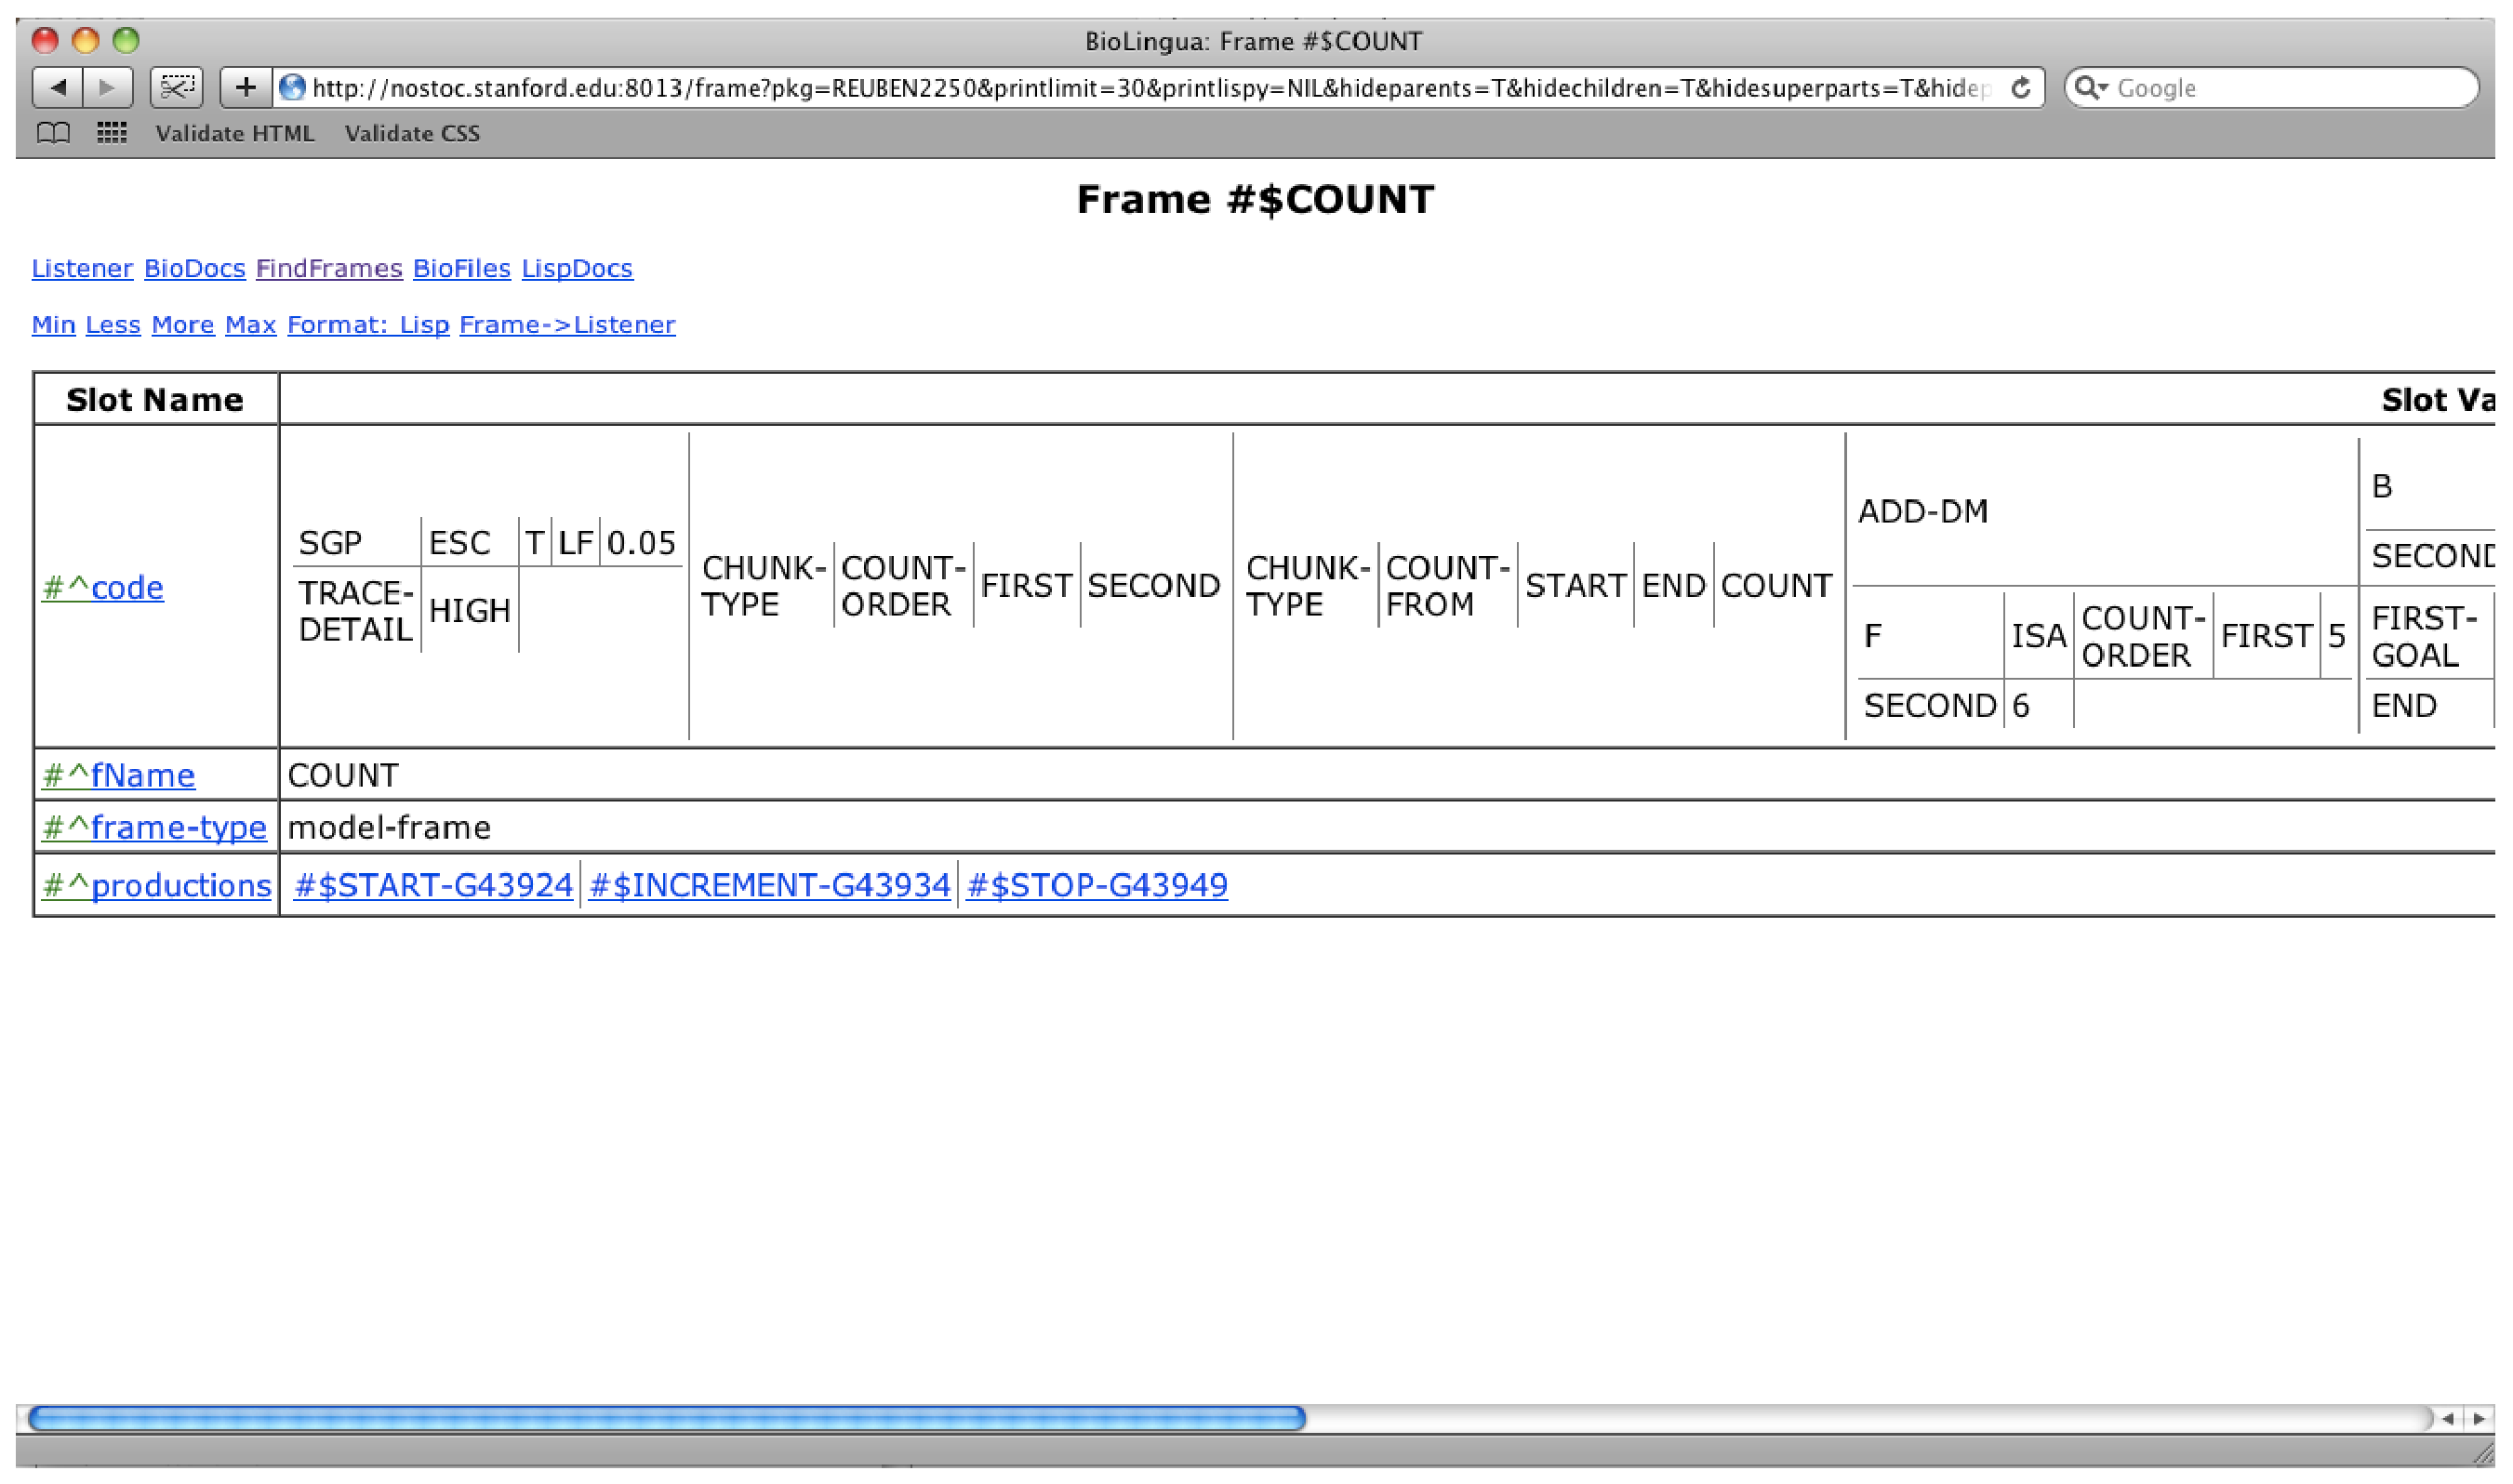
\includegraphics[width=100mm]{NavigateFrame}
  \caption{Navigating a model represented as a frame}
  \label{NavigateFrame}
\end{figure}

\begin{figure}[htp]
  \centering
  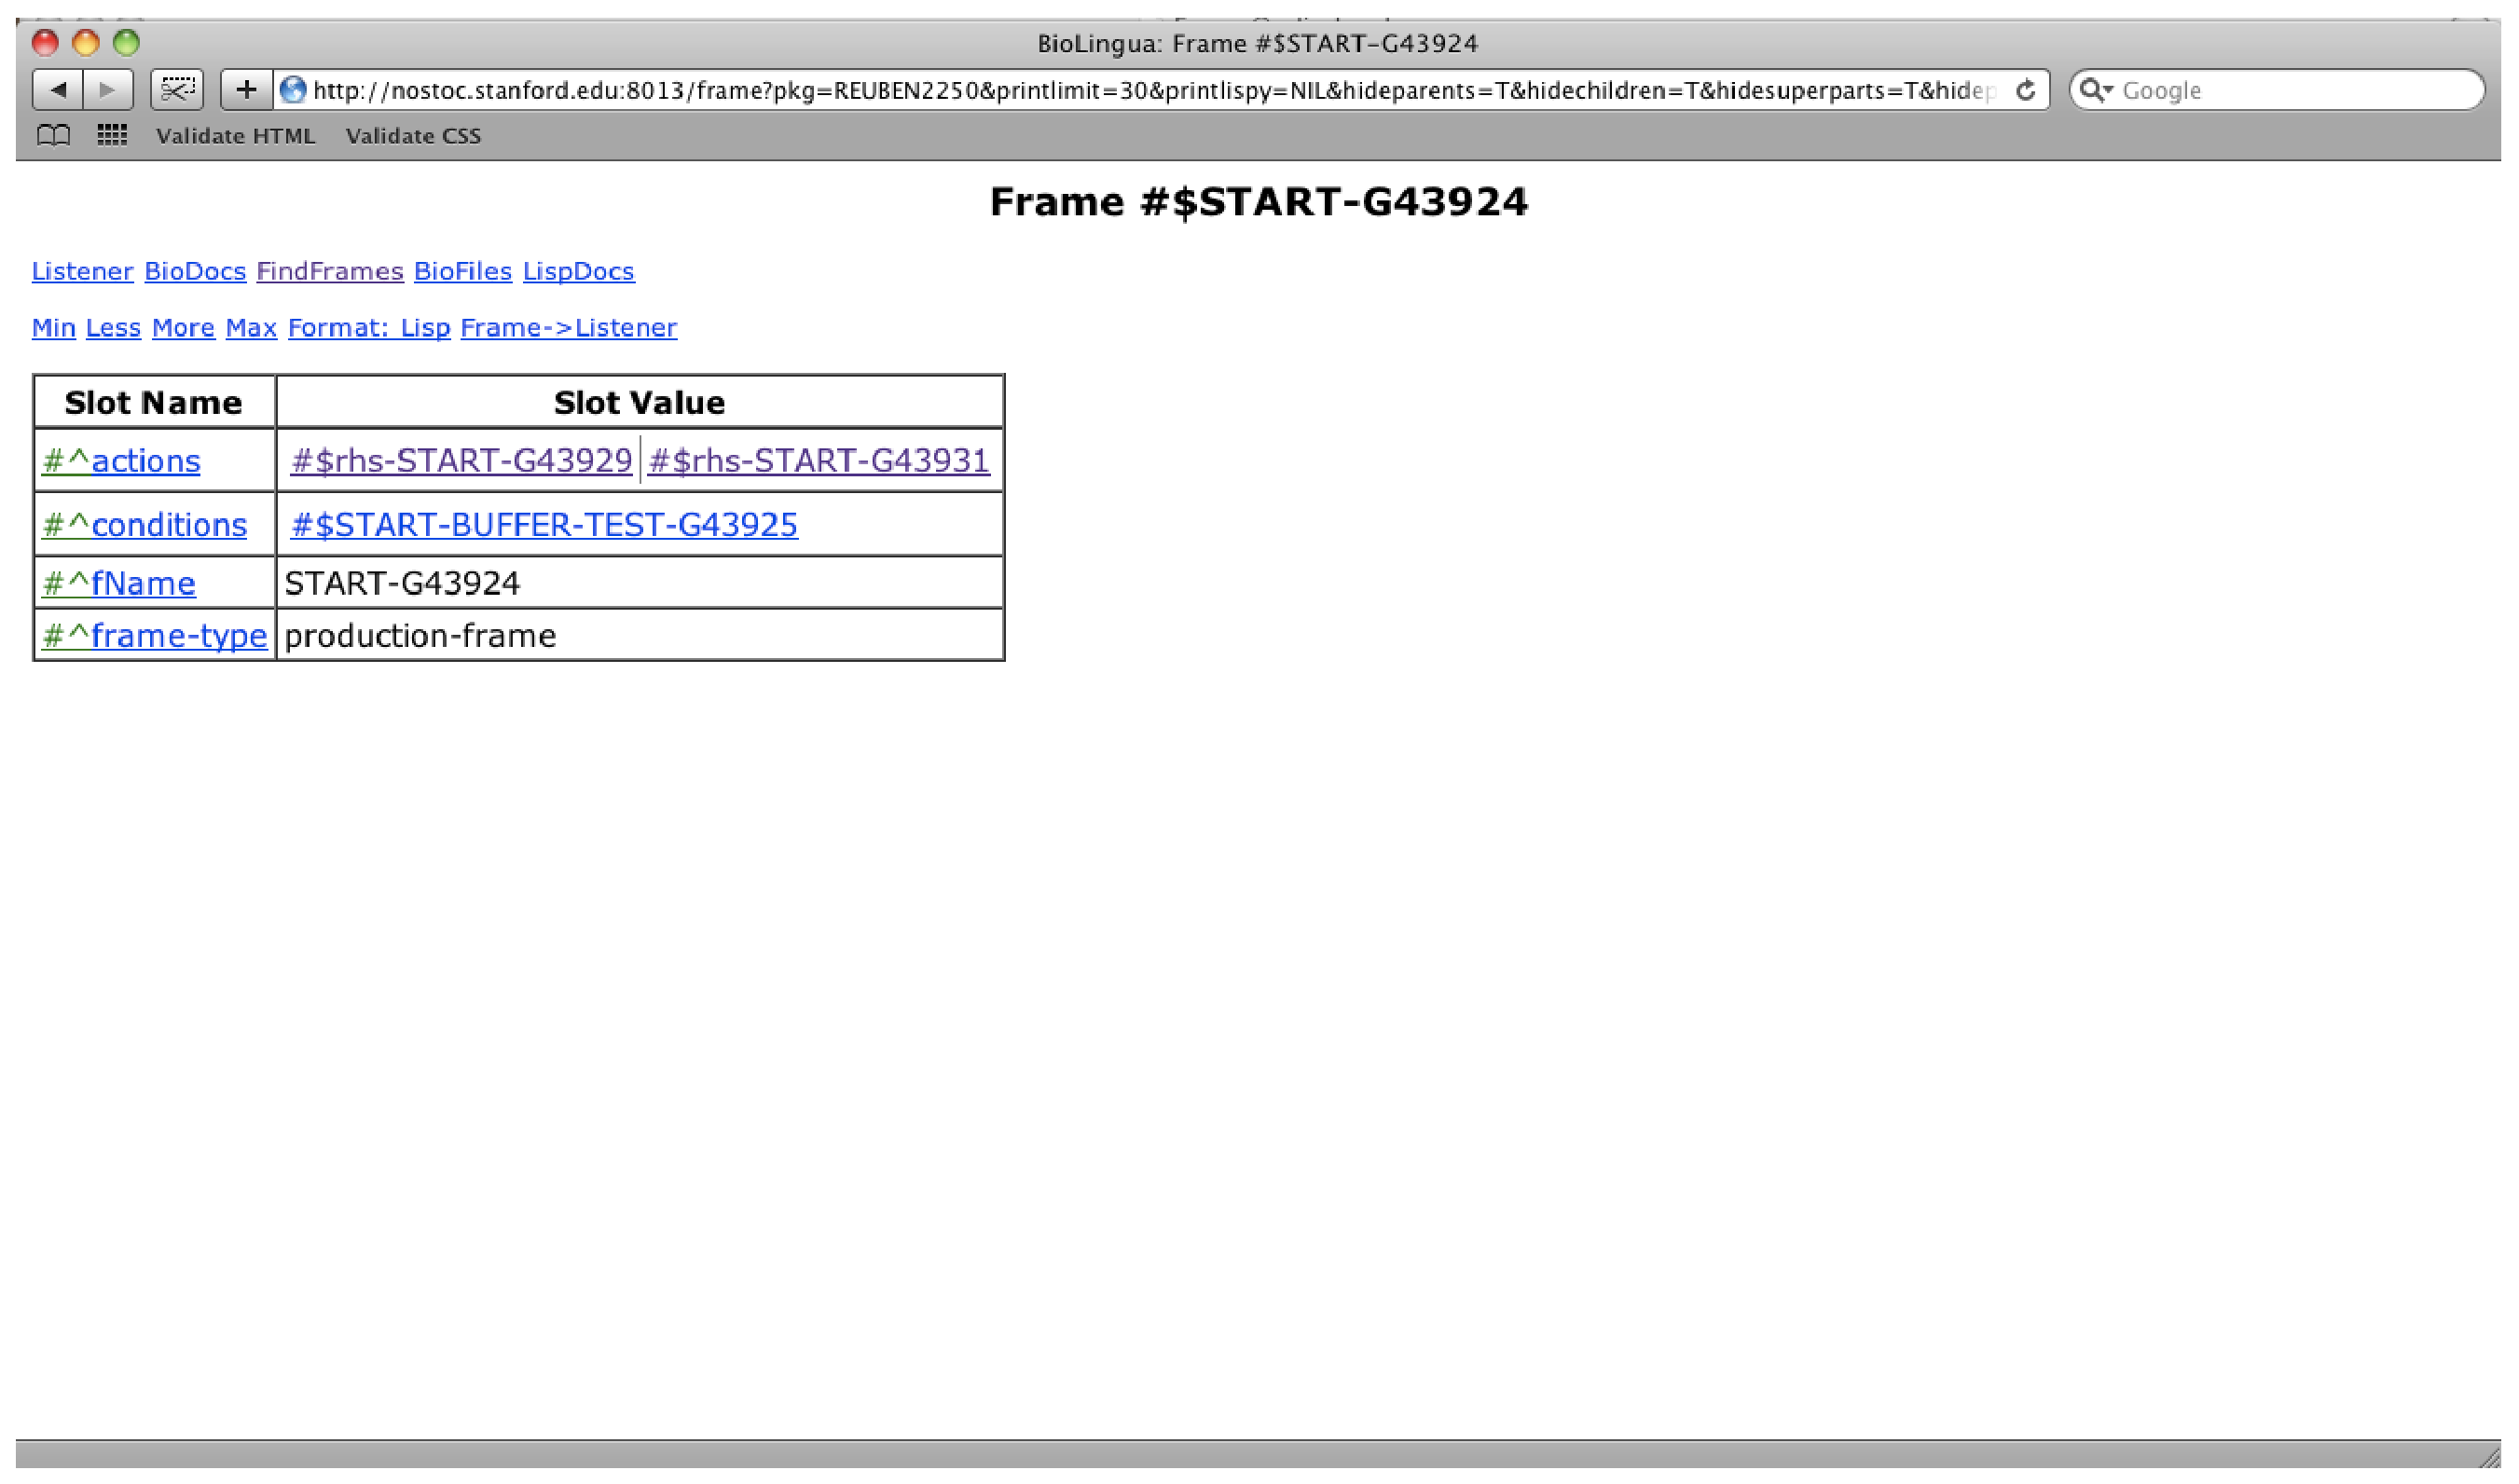
\includegraphics[width=100mm]{NavigatingAProduction}
  \caption{Navigating a production represented as a frame}
  \label{NavigatingAProduction}
\end{figure}

\begin{figure}[htp]
  \centering
  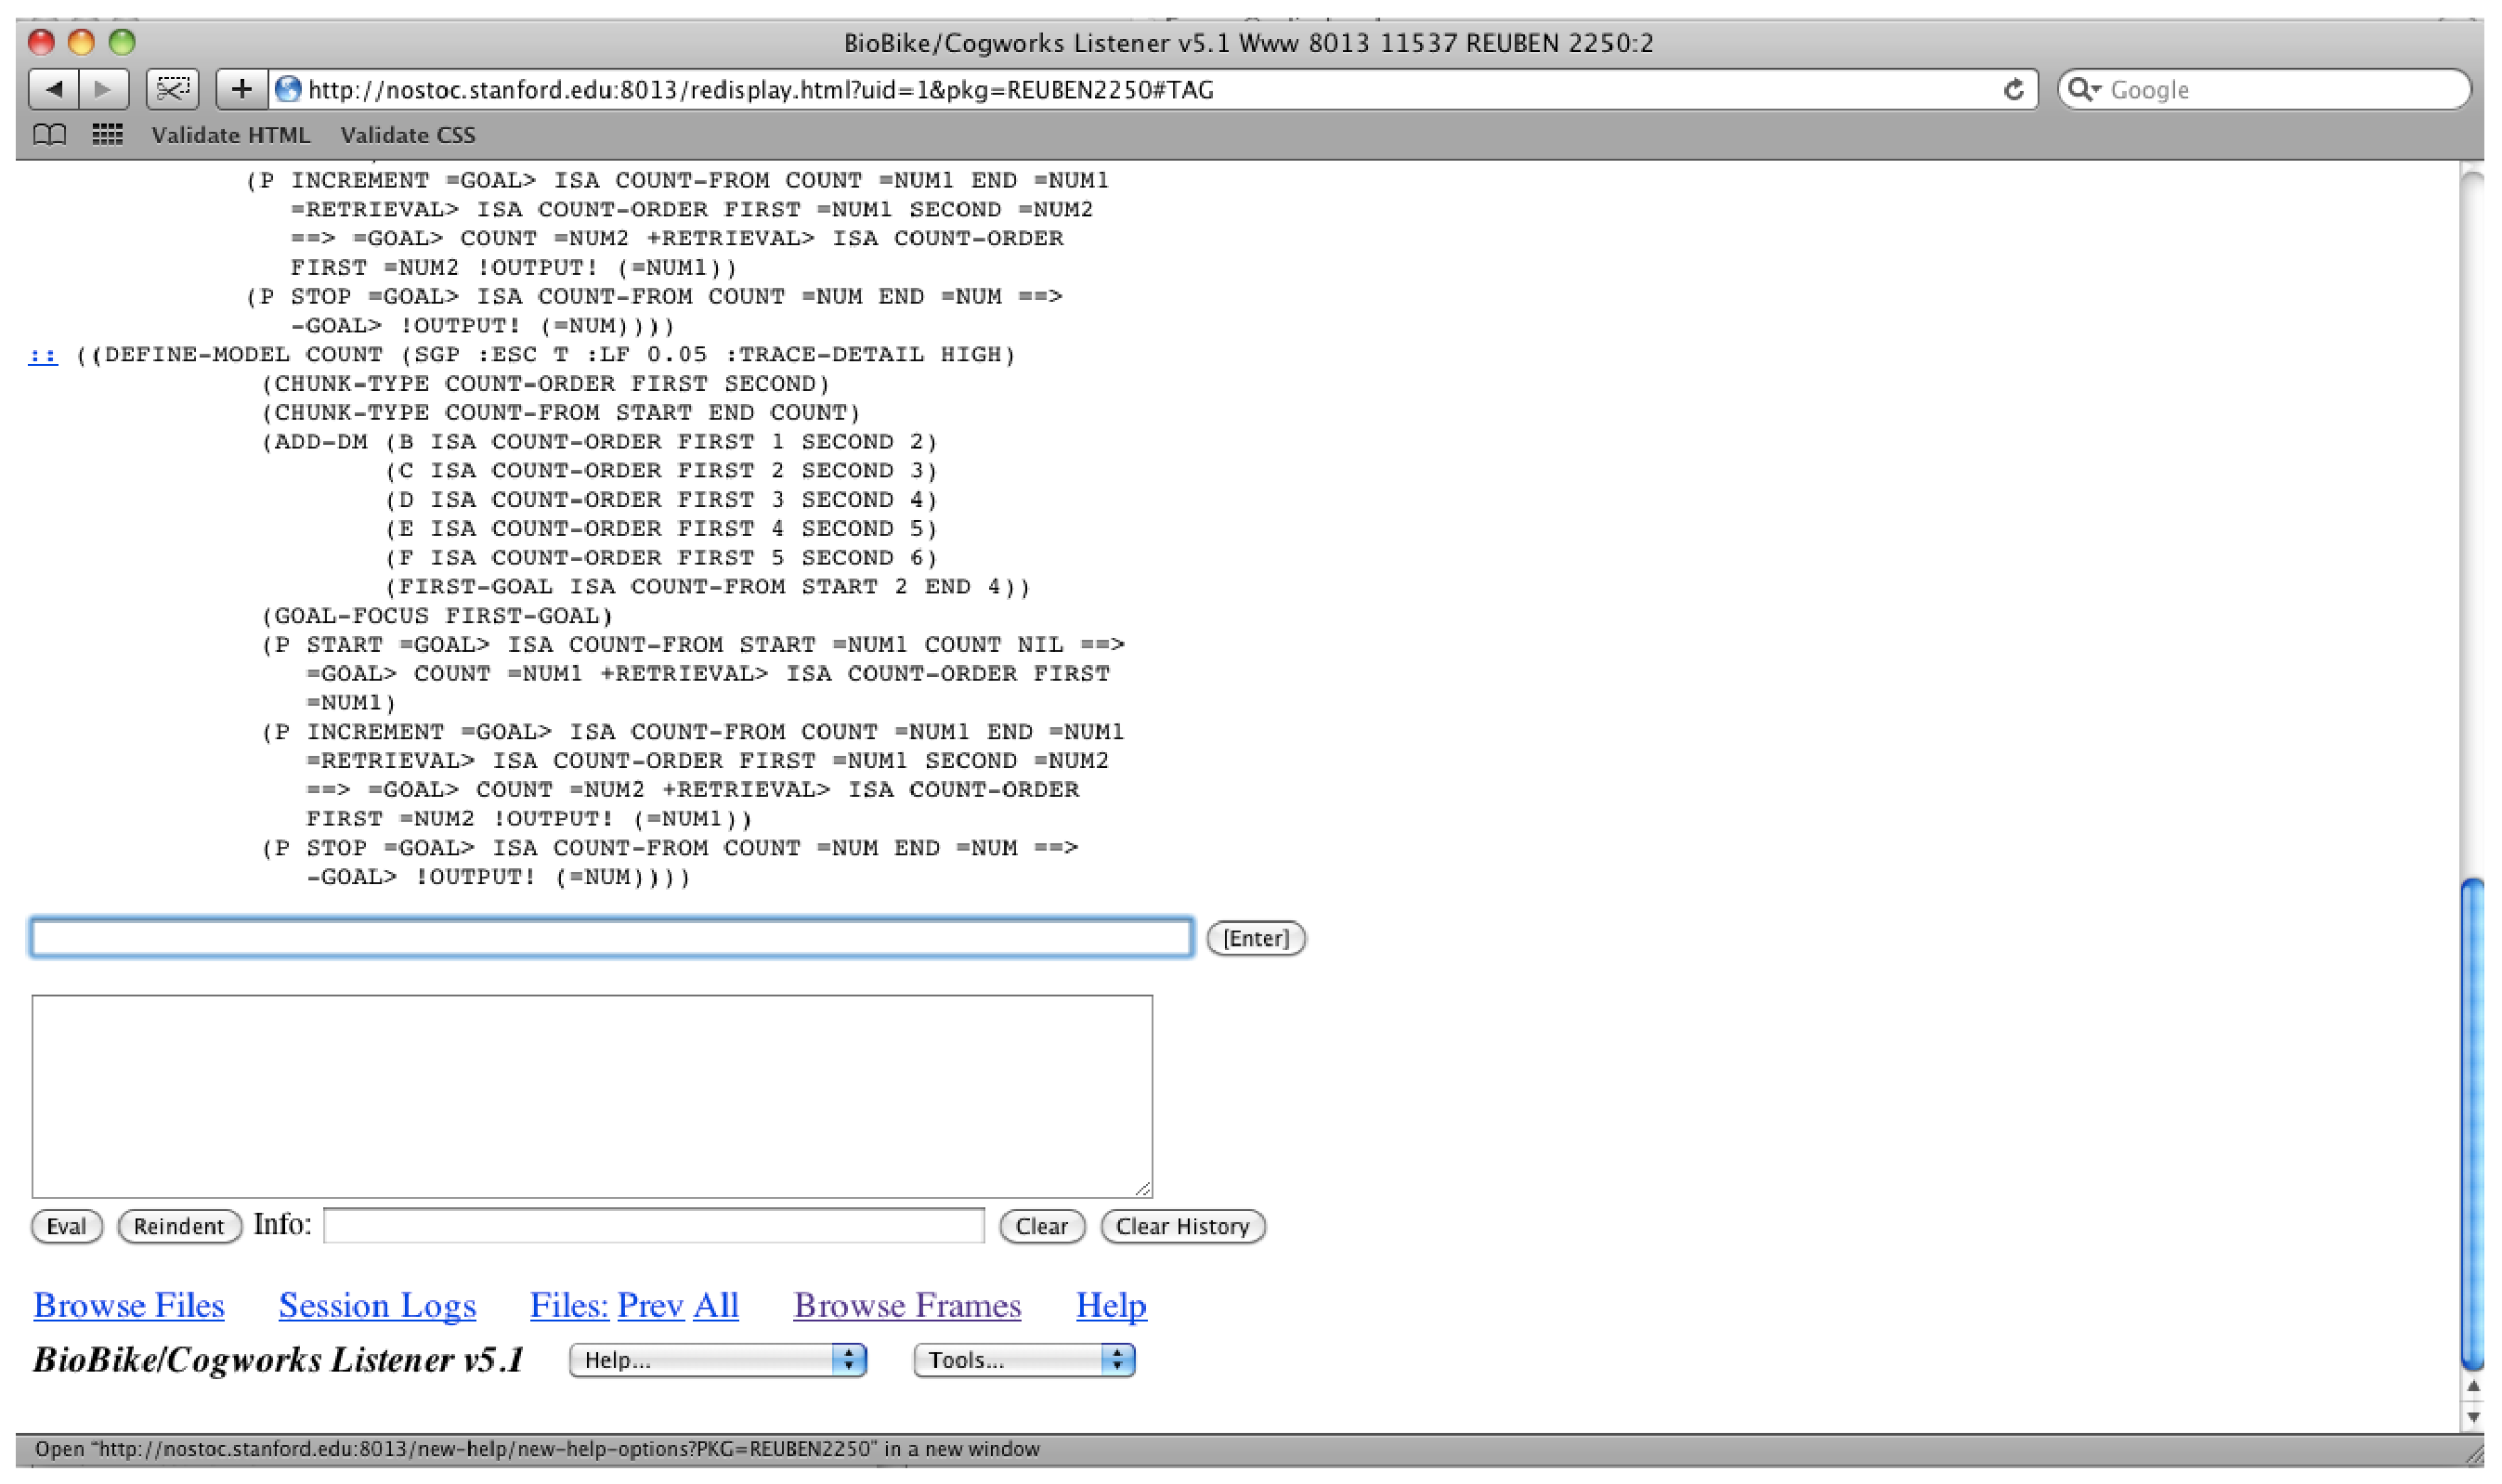
\includegraphics[width=100mm]{ConvertFrameToImage}
  \caption{The resultant code after clicking the Frame $->$ Listener
    link}
  \label{ConvertFrameToImage}
\end{figure}

As can be seen from the work flow building a model and sharing the
same with other users is as intuitive as it can be.

% Coglaborate
%       - Describe work flow that shows collaboration occurs with screen shots.
%       - Describe what was modified and why
%         - Describe how frames are created
%         - Describe how the reverse procedure is implemented

\section{Proof of concept}
% Proof of concept
%        - Problem description
%        - Approaches
%        - Approach taken
%        - What can be deduced from it.

